\section{Frequency lock to a spectroscopic line with LIA module }

An easy way to stabilize the frequency of a laser is to lock its frequency to an atomic or molecular transition.
An advantage of this method is that the optical transitions can be quite narrow, typically on the order of a few MHz, however, the thermal Doppler broadening will considerably increase the width of these transitions.

To avoid the Doppler broadening effect, an optical scheme such as the one shown in fig. ~\ref{fig:spectroscopic-line-lock} can be used, saturation spectroscopy allows to achieve a sub-Doppler resolution in order to identify the central frequency of the transition with more precision.

The laser beam to be stabilized is divided into two parts using a beam splitter. Most of the laser radiation is transmitted and is called "pump" beam, a small fraction of the laser radiation is reflected and is called "probe" beam. 
The two beams have counter-propagating paths and overlap in the cell containing the reference gas.
The probe beam is detected after the cell by a photodetector.

This configuration allows to identify the Lamb dip, result of the saturated absorption process,and using a common modulation spectroscopy technique it is possible to obtain the error signal for the laser frequency correction.

\begin{figure}[H]
\centering
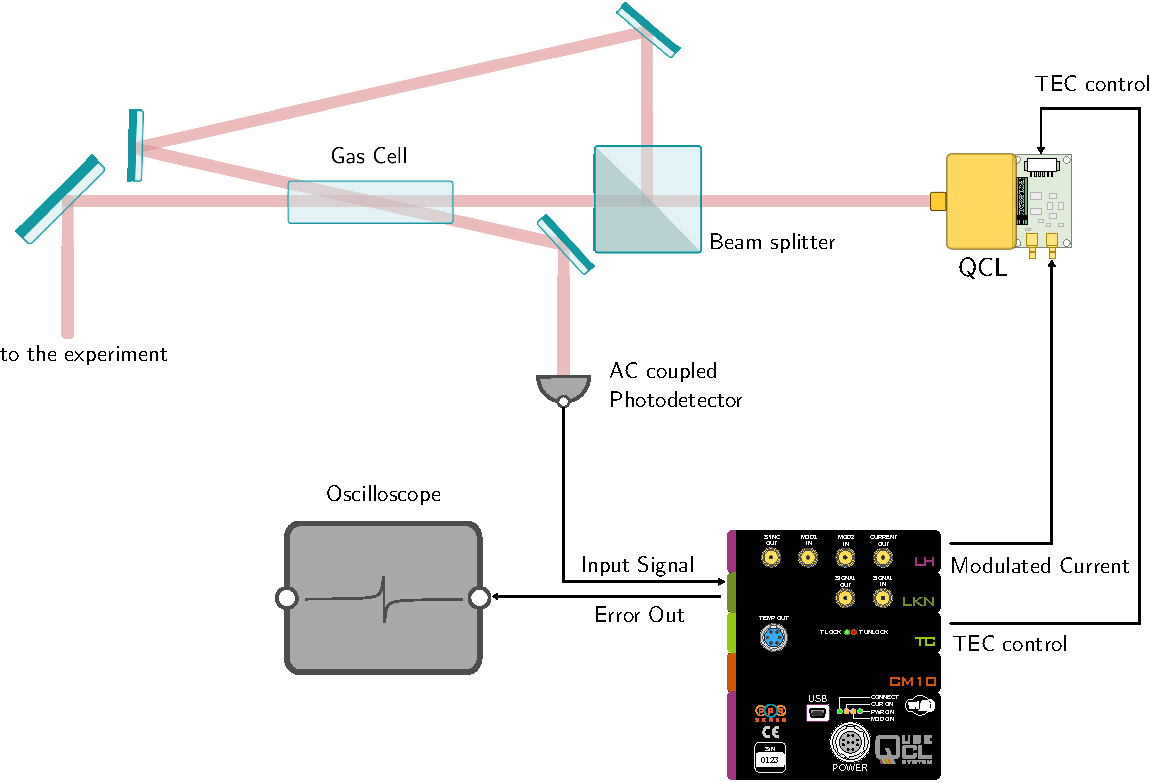
\includegraphics[width=12cm]{images/LKN_EXPERIMENT_DEMO.pdf}
\caption{spectroscopic line lock using LIA module}
\label{fig:spectroscopic-line-lock}
\end{figure}
\newpage
Using the lock-in module (LIA) installed on the \QubeModel  System, it is possible to directly acquire the spectroscopy signal from the photodetector and apply the correction to the laser for frequency locking.
In this configuration, the \QubeModel  is able to perform internally all the necessary operations to control the locking procedure:
\begin{itemize}
    \item[1.]Current modulation with frequency and amplitude control
    \item[2.]Signal demodulation with amplification and integration-time control
    \item[3.]Processing of the error signal by using a PID controller 
    \item[4.]Addition of the correction current directly to the laser bias current
\end{itemize}


The Qube Control Software allows to keep under control all the parameters for the optimization of the locking procedure.

\begin{figure}[H]
\centering
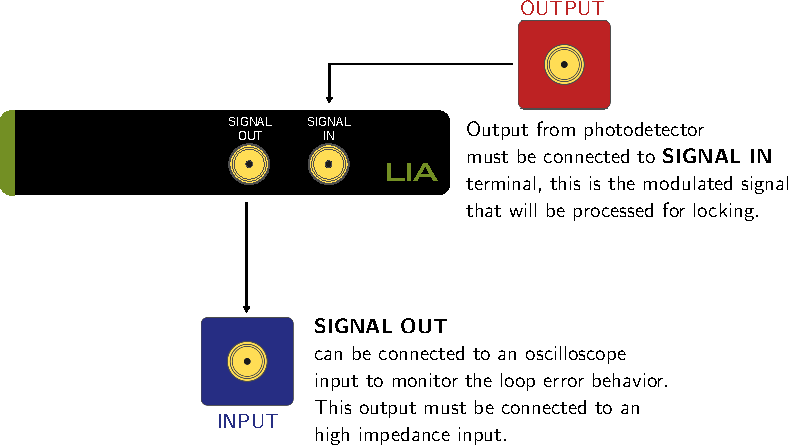
\includegraphics[width=12cm]{images/LIA_INPUT_EXPLANATION.pdf}
\caption{LIA terminals explanation}
\end{figure}




\newpage
\section{Offset phase lock with PLL module}

Frequency locking between two lasers is a technique for transferring the frequency and phase characteristics of a reference laser to a target laser.

It is commonly used in spectroscopic applications and in metrology.
\newline
The figure shows a possible optical scheme for an implementation of an offset phase lock between two Quantum Cascade Lasers anyway the \QubeModel  System can work with any type of diode laser.
\begin{figure}[H]
\centering
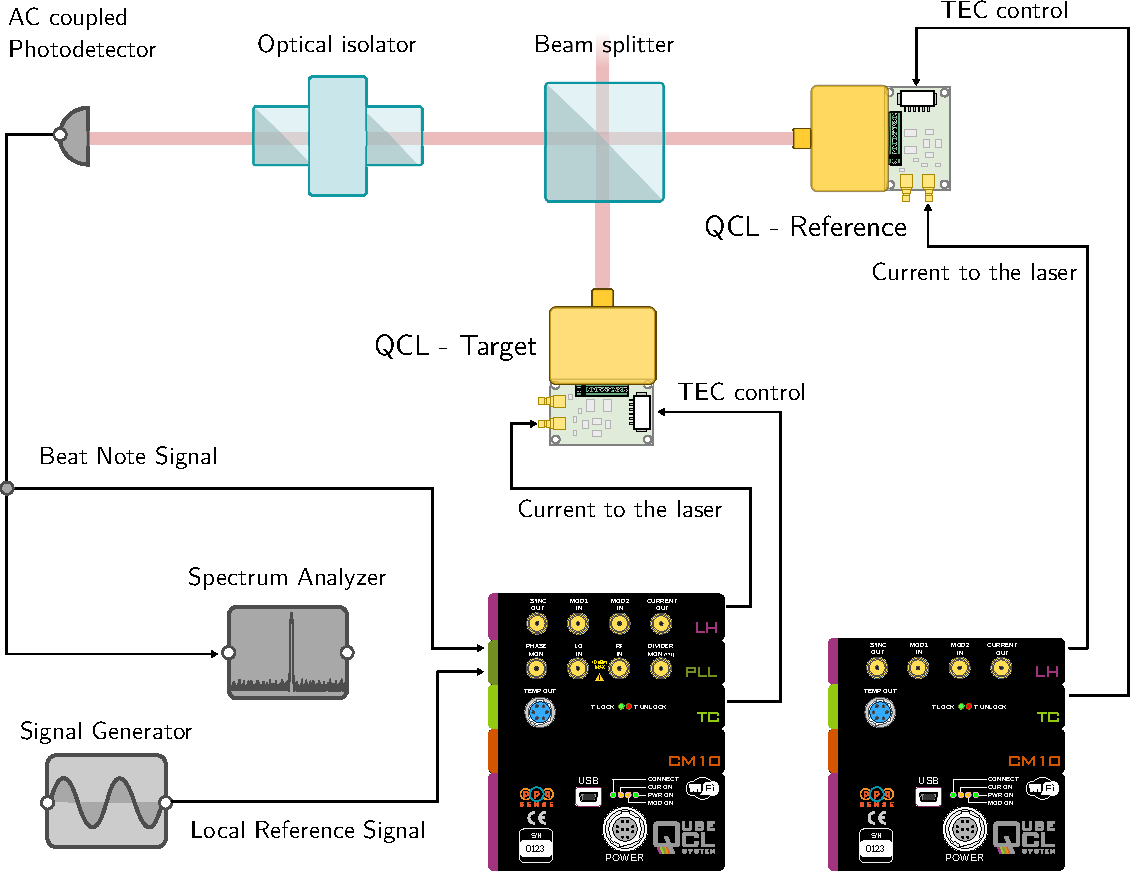
\includegraphics[width=12cm]{images/PLL_EXPERIMENT_DEMO.pdf}
\caption{PLL laser lock setup}
\end{figure}
The reference light is superimposed on the target light using a beam splitter.

The overlap of the beams is detected with a wide band photodiode and generates a beat signal at the frequency difference between the target light and the reference,
the beat-note frequency is usually in the hundreds of MHz.

The beat-note frequency is a function of the phase difference between the target light and the optical reference and it is constant only if the frequency difference between the target light and the reference light is exactly zero, any phase change will result in a variation of the signal.

To perform an offset lock, the beat note is mixed with a local RF reference  signal with frequency $\omega_{offset}$, 
at this point the signal obtained from this procedure will be constant only if the frequency difference between the target light and the optical reference is exactly $\omega_{offset}$, this is the final error signal used for offset frequency locking.

Using the PLL module integrated in the QuebeCL System, it will be sufficient to send the photodiode signal to the RF IN input and the module will add the correction signal directly to the laser current for frequency/phase stabilization, through the Qube Control Software it is possible to keep under control all the parameters for the optimization of the locking procedure.

\begin{figure}[H]
\centering
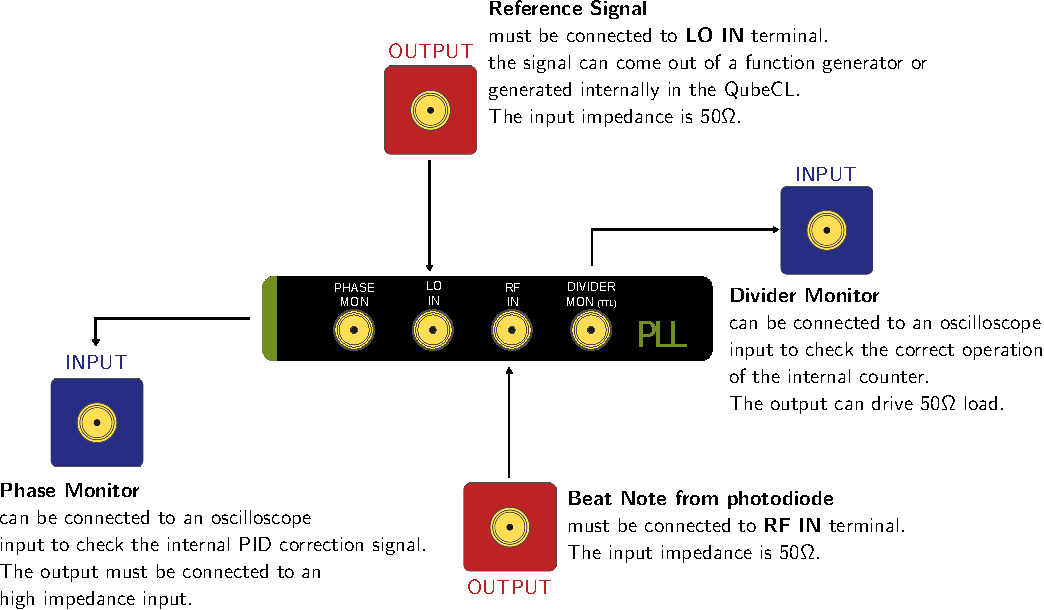
\includegraphics[width=12cm]{images/PLL_INPUT_EXPLANATION.pdf}
\caption{PLL terminals explanation}
\end{figure}


\newpage
\section{High finesse cavity lock with PDH module}

The Pound-Drever-Hall technique is a method to match the emitting optical frequency of a laser to a resonance of a Fabry-Perot cavity.
However stable the laser and cavity may be, both the length of the cavity and the frequency of the laser vary over time.
PDH locking technique uses the light reflected from the cavity to create an error signal that can be used to correct the laser frequency or change the length of the cavity so that they stay matched and transmission is maximized.

In the PDH technique the laser frequency is modulated, modulated light consists of a carrier frequency and two sidebands.
The light reflected from the cavity is measured using a fast photodetector, the reflected signal consists of the two unaltered sidebands together with an out-of-phase carrier component.
\newline
The photodetector signal is mixed with a local oscillator, which is in phase with the light modulation. After phase shift and filtering, the resulting electronic signal has a dispersive line shape that can be used as error signal for active stabilization.

For high-fineness cavities, the frequency spacing of the sidebands can be of the order of MHz, in this situation the modulation can be applied directly on the laser current, without the need for external electro-optical modulators.


\begin{figure}[H]
\centering
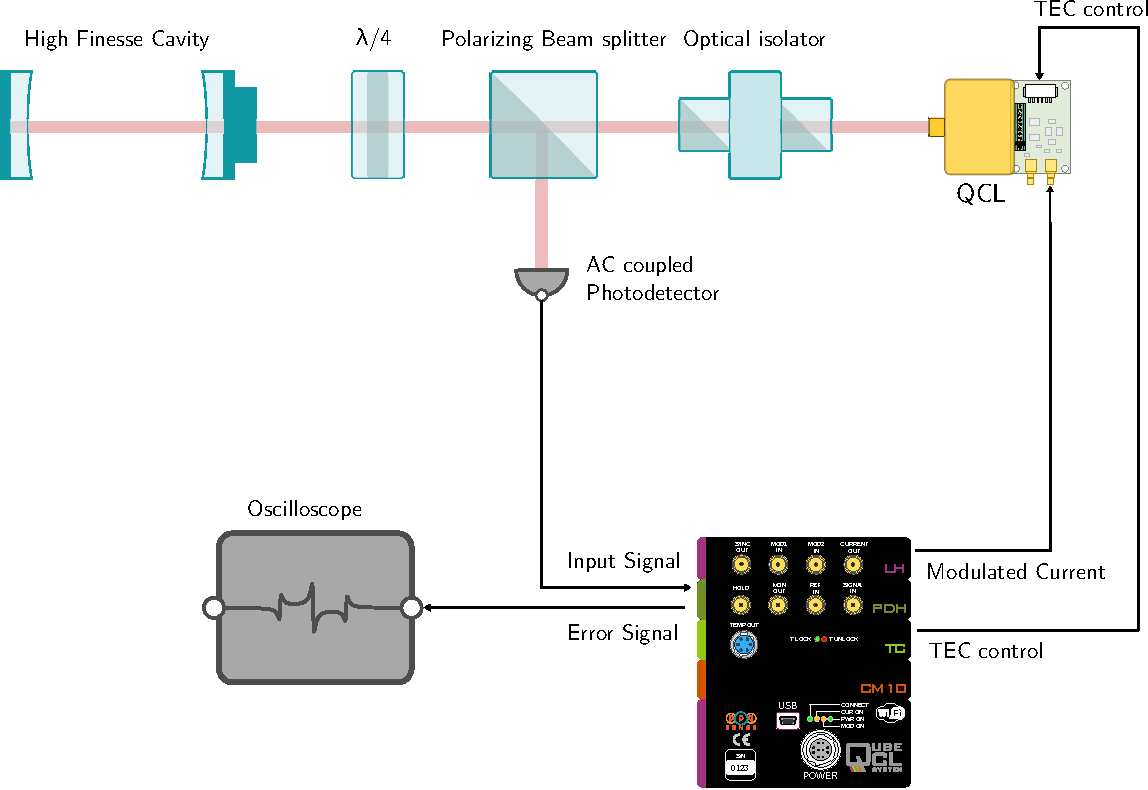
\includegraphics[width=12cm]{images/PDH_EXPERIMENT_DEMO.pdf}
\caption{PDH cavity lock setup}
\end{figure}

The PDH module accepts in input directly the signal coming from the photodiode, processes it and applies the correction to perform the lock directly on the laser current. The  Qube Control Software allows to keep under control all the parameters for the optimization of the locking procedure.

\begin{figure}[H]
\centering
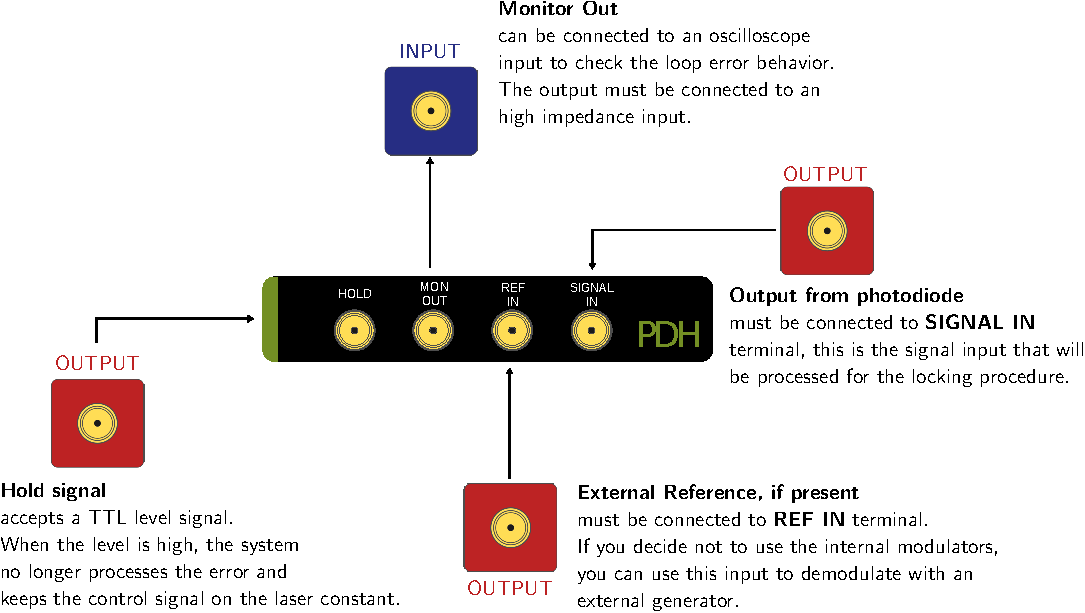
\includegraphics[width=12cm]{images/PDH_INPUT_EXPLANATION.pdf}
\caption{PDH terminals explanation}
\end{figure}

